
\documentclass{article}

\usepackage{graphicx}
\usepackage{listings}
\usepackage{flexisym}
\usepackage{graphicx}

\graphicspath{ {images/} }

\begin{document}

  \title{ECE 375: Assignment 1}
  \author{Jared Wasinger}

  \maketitle
  \begin{enumerate}
  \item Write a regular expression for all strings of letters that come from the alphabet $\sigma=\{a,b\}$ that start with either \textbf{aa} or \textbf{bb}, followed by a string of 0 or more b's, and ends with a single a [10 points]\\

  $(aa|bb)b^*a$\\

  \item Using Thompson's Construction, create a NFA that accepts the strings from the regular expression above. [10 points]\\
  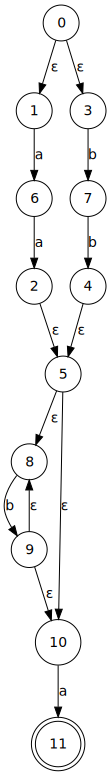
\includegraphics{nfa.png}\\

  \item Using the Subset Construction, create a DFA from the NFA above. [10 points]\\
  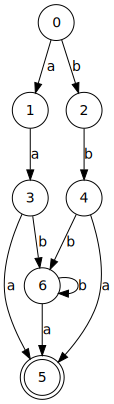
\includegraphics{dfa.png}\\

  \item Try to merge states to get the smallest machine possible.  When you merge states, provide a justification for why the states may be merged. [10 points]
  \end{enumerate}
\end{document}
